
\begin{frame}{Example - drone trajectory, 1}
	\begin{flushleft}
		
		Consider the following problem: plan a dynamics-consistent trajectory for a quadrotor as a quadratic program.
		
		\bigskip
		
		This can be solved by using a simplified dynamical model of a drone, based on \emph{differential flatness}. The essential idea is to plan position, velocity, acceleration, and jerk of the center of mass (CoM) of the drone, and recover the orientation and angular velocity from this information:
		
		\begin{itemize}
			\item Knowing acceleration you can compute thrust.
			\item Knowing thrust, you can compute orientation (up to yaw).
			\item Knowing jerk you can compute angular velocity.
		\end{itemize}
		
	\end{flushleft}
\end{frame}



\begin{frame}{Example - drone trajectory, 2}
	\begin{flushleft}
		
		Let $\bo{B} = [\bo{b}_1 \ \bo{b}_2 \ \bo{b}_3]$ be a rotation matrix, describing the orientation of the quadrotor in the world frame.
		
		\begin{figure}
			\centering
			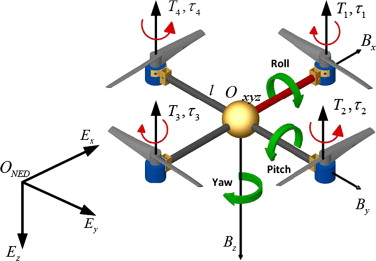
\includegraphics[width=0.6\linewidth]{quadrotor_planning}
			%\caption{Quadrotor body frame}
			\label{fig:drone}
		\end{figure}
		
		 We use the following convention: $\bo{b}_1$ and $\bo{b}_2$ lie in the tangent plane of the drone, and $\bo{b}_3$ lies in the normal direction to the plane; these vectors are chosen such that they form a right-handed basis and the thrust $\bo{f}_t = -f \bo{b}_3$ (vector $\bo{b}_3$ "points down" in the body frame).
		
	\end{flushleft}
\end{frame}



\begin{frame}{Example - drone trajectory, 3}
	\begin{flushleft}
		
		We know that gravity in the world frame is expressed as $\bo{f}_g = mg \bo{e}_3$, where $\bo{e}_3 = [0 \ 0 \ 1 ]\T$ (also "points down") and $g \approx 9.81$.
		
		\bigskip
		
		The accelepation of the CoM can be computed as:
		%
		\begin{align}
			m \bo{a} = \bo{f}_g + \bo{f}_t 
			\\
			\bo{f}_t = m (\bo{a} - g \bo{e}_3)
		\end{align}
		%
		$\bo{b}_3$ is the opposite direction to $\bo{f}_t$ and unit length:
		%
		\begin{align}
			 \bo{b}_3 = -\frac{\bo{f}_t}{||\bo{f}_t||} =  \frac{g \bo{e}_3 - \bo{a}}{||g \bo{e}_3 - \bo{a}||}
		\end{align}
		%
		
		
		
	\end{flushleft}
\end{frame}


\begin{frame}{Example - drone trajectory, 4}
	\begin{flushleft}
		
		Thus, our decision variables are position $\bo{p}$, velocity $\bo{v} = \dot{\bo{p}}$, acceleration $\bo{a} = \ddot{\bo{p}}$, and jerk $\bo{j} = \dddot{\bo{p}}$. 
		
		\bigskip
		
		In our optimization, we can aim to minimize snap (4-th derivative of position, derivative of jerk). The cost function will then take form:
		
		\begin{equation}
			\boxed{
			J = \sum_{i = 1}^{N-1} ( \bo{j}_{i+1} - \bo{j}_i)\T ( \bo{j}_{i+1} - \bo{j}_i) }
		\end{equation}
		
		
	\end{flushleft}
\end{frame}



\begin{frame}{Example - drone trajectory, 5}
	\begin{flushleft}
		
		{\small 
		We can add constraints; for example, we can require a certain pitch-roll at the time step $k$. To do that, we describe the desired pitch-roll pair via desired normal direction $\bo{b}_3^\text{des}$ (the desired orientation of the quadrotor's vertical axis). 
		
		The constraint then can be written as "the cross product between $\bo{b}_3$ and $\bo{b}_3^\text{des}$ should be zero":
		%
		\begin{align}
			\bo{b}_3^\text{des} \times \bo{b}_3 = 0
			\\
			\bo{b}_3^\text{des} \times   \frac{g \bo{e}_3 - \bo{a}}{||g \bo{e}_3 - \bo{a}||} = 0
			\\
			\boxed{
			\bo{b}_3^\text{des} \times (g \bo{e}_3 - \bo{a}) = 0
		}
		\end{align} 
		%
		To avoid the scenaro where $\bo{b}_3$ is facing teh opposite direction to $\bo{b}_3^\text{des}$, we can add a constraint:
		%
		\begin{align}
			(\bo{b}_3^\text{des} )\T  \bo{b}_3 \geq 0
			\\
			\boxed{
				(\bo{b}_3^\text{des} )\T (g \bo{e}_3 - \bo{a}) \geq 0
			}
		\end{align} 
		
	}
	\end{flushleft}
\end{frame}



\begin{frame}{Example - drone trajectory, 6}
	\begin{flushleft}
		
		Adding constraints on the initial and final positions, the trajectory planning problem becomes a QP:
		
		\begin{equation}
			\begin{aligned}
				& \underset{\bo{p},\bo{v},\bo{a},\bo{j}}{\text{minimize}}
				& &\sum_{i = 1}^{N-1} ( \bo{j}_{i+1} - \bo{j}_i)\T ( \bo{j}_{i+1} - \bo{j}_i), \\
				& \text{subject to}
				& & \begin{cases}
					\bo{b}_3^\text{des}(k) \times (g \bo{e}_3 - \bo{a}_k) = 0
					\\
					(\bo{b}_3^\text{des} )\T (g \bo{e}_3 - \bo{a}) \geq 0,
					\\
					\bo{p}_{i+1} = \bo{p}_i + h \bo{v}_i \\
					\bo{v}_{i+1} = \bo{v}_i + h \bo{a}_i \\
					\bo{a}_{i+1} = \bo{a}_i + h \bo{j}_i 
					\\
					\bo{p}_1 = \bo{p}_1^\text{des}
					\\
					\bo{p}_N = \bo{p}_N^\text{des}
				\end{cases}
			\end{aligned}
		\end{equation}
		%
		where $h$ is the time step.
		
	\end{flushleft}
\end{frame}



\begin{frame}{Example - drone trajectory, 7 (extra)}
	\begin{flushleft}
		
		
		To compute orientation $\bo{B} = [\bo{b}_1 \ \bo{b}_2 \ \bo{b}_3]$ from $\bo{a}$ we use the following steps:
		
		\begin{enumerate}
			
			\item Compute $\bo{b}_3 =  \frac{g \bo{e}_3 - \bo{a}}{||g \bo{e}_3 - \bo{a}||}$.
			
			\item Choose yaw reference $\psi$ and $\bo{b}_\text{yaw} = \begin{bmatrix}
			\cos (\psi) & \sin(\psi) & 0
			\end{bmatrix}\T$.
			
			\item Compute $\bo{b}_2$ via orthogonality and normalization: $\bo{b}_2 = \frac{\bo{b}_3 \times \bo{b}_\text{yaw}}{||\bo{b}_3 \times \bo{b}_\text{yaw}||}$
			
			\item Finish the basis $\bo{b}_1 =  \bo{b}_2 \times \bo{b}_3$.
		\end{enumerate}
		
	\end{flushleft}
\end{frame}



\begin{frame}{Example - drone trajectory, 8 (extra)}
	\begin{flushleft}
		
		
		To compute angular velocity (local frame) $\omega = \begin{bmatrix}
		\omega_x & \omega_y & \omega_z
		\end{bmatrix}\T$ from $\bo{j}$ we use the following steps:
		
		\begin{enumerate}
			
			\item Compute $\dot{ \bo{b}}_3 =  -\frac{1}{||g \bo{e}_3 - \bo{a}||}(\bo{I} - \bo{b}_3 \bo{b}_3\T) \bo{j}$. \textcolor{mygray}{ We use the fact that $\bo{b}_3 = -\frac{\bo{f}_t}{||\bo{f}_t||}$ is a unit vector.}
			
			\item Compute $\omega_x = - \bo{b}_2\T \dot{ \bo{b}}_3$ and $\omega_y = \bo{b}_1\T \dot{ \bo{b}}_3$.
			
			\item Choose $\omega_z = \dot \psi$.
		\end{enumerate}
		
		\bigskip
		
		\textcolor{mygray2}{
		Note that $\omega = \omega_x \bo{b}_1 + \omega_y \bo{b}_2+ \omega_z \bo{b}_3$, hence $\dot{ \bo{b}}_3  = \omega \times \bo{b}_3 = ( \omega_x \bo{b}_1 + \omega_y \bo{b}_2) \times \bo{b}_3$. Since $ \bo{b}_1 \times  \bo{b}_3 =  -\bo{b}_2$ and $ \bo{b}_2 \times  \bo{b}_3 =  \bo{b}_1$ we get $\dot{ \bo{b}}_3  =  -\omega_x \bo{b}_2+ \omega_y \bo{b}_1$. Projecting we get the formulas above.}
		
	\end{flushleft}
\end{frame}